\section{Dynamic Linear Models (DLM)}

A DLM is specified by the following equations:

\begin{equation*}
    \begin{cases}
        y_t = F_t\theta_t + \nu_t, \quad &\nu_t \sim \text{N}(0,V_t) \\
        \theta_t = G_t\theta_{t-1} + \omega_t, \quad &\omega_t \sim \text{N}(0, W_t)
    \end{cases}
\end{equation*}

for $t = 1, \dots, n$ together with a prior distribution for $\theta_0$:

\begin{equation*}
    \theta_0 \sim \text{N}(m_0, C_0)
\end{equation*}
\nline
Here $y_t$ is an $m$-dimensional vector, representing the observation at time $t$, while $\theta_t$ is a generally unobservable $p$-dimensional vector representing the state of the system at time $t$. The $\nu_t$’s are observation errors and the $\omega_t$’s evolution errors. The matrices $F_t$ and $G_t$ have dimension $m$ by $p$ and $p$ by $p$, respectively, while $V_t$ and $W_t$ are variance matrices of the appropriate dimension.

\subsection{Building the model}

Here we let our prior consist of a second order polynomial and seasonal$^4$ component.
\nline
After fitting a model to our data and smoothing we are able to extract the follow plots shown in \autoref{S3fig:trend}. We can see our model has estimated a strong seasonal component and a downward trend.
\nline
Using our model we are able to apply a filter and then produce a forecast 6 quarters past our data, this is shown in \autoref{S3fig:Forecast}. Comparing the forecast produced using DLM to our ARMA model, \autoref{S2fig:ARMA forecast} we can see that the 95\% confidence interval is smaller for DLM implying that it is more confident in its prediction. It is also worth noting that the ARMA forecast has uniform error margins, whereas in the DLM forecast the error bars get larger as the forecast moves further into the future. The DLM forecast also takes on a very different shape proceeding with a slight continuous increase opposed to the big rises and falls predicted by the ARMA model.

\begin{figure}[H]
    \centering
    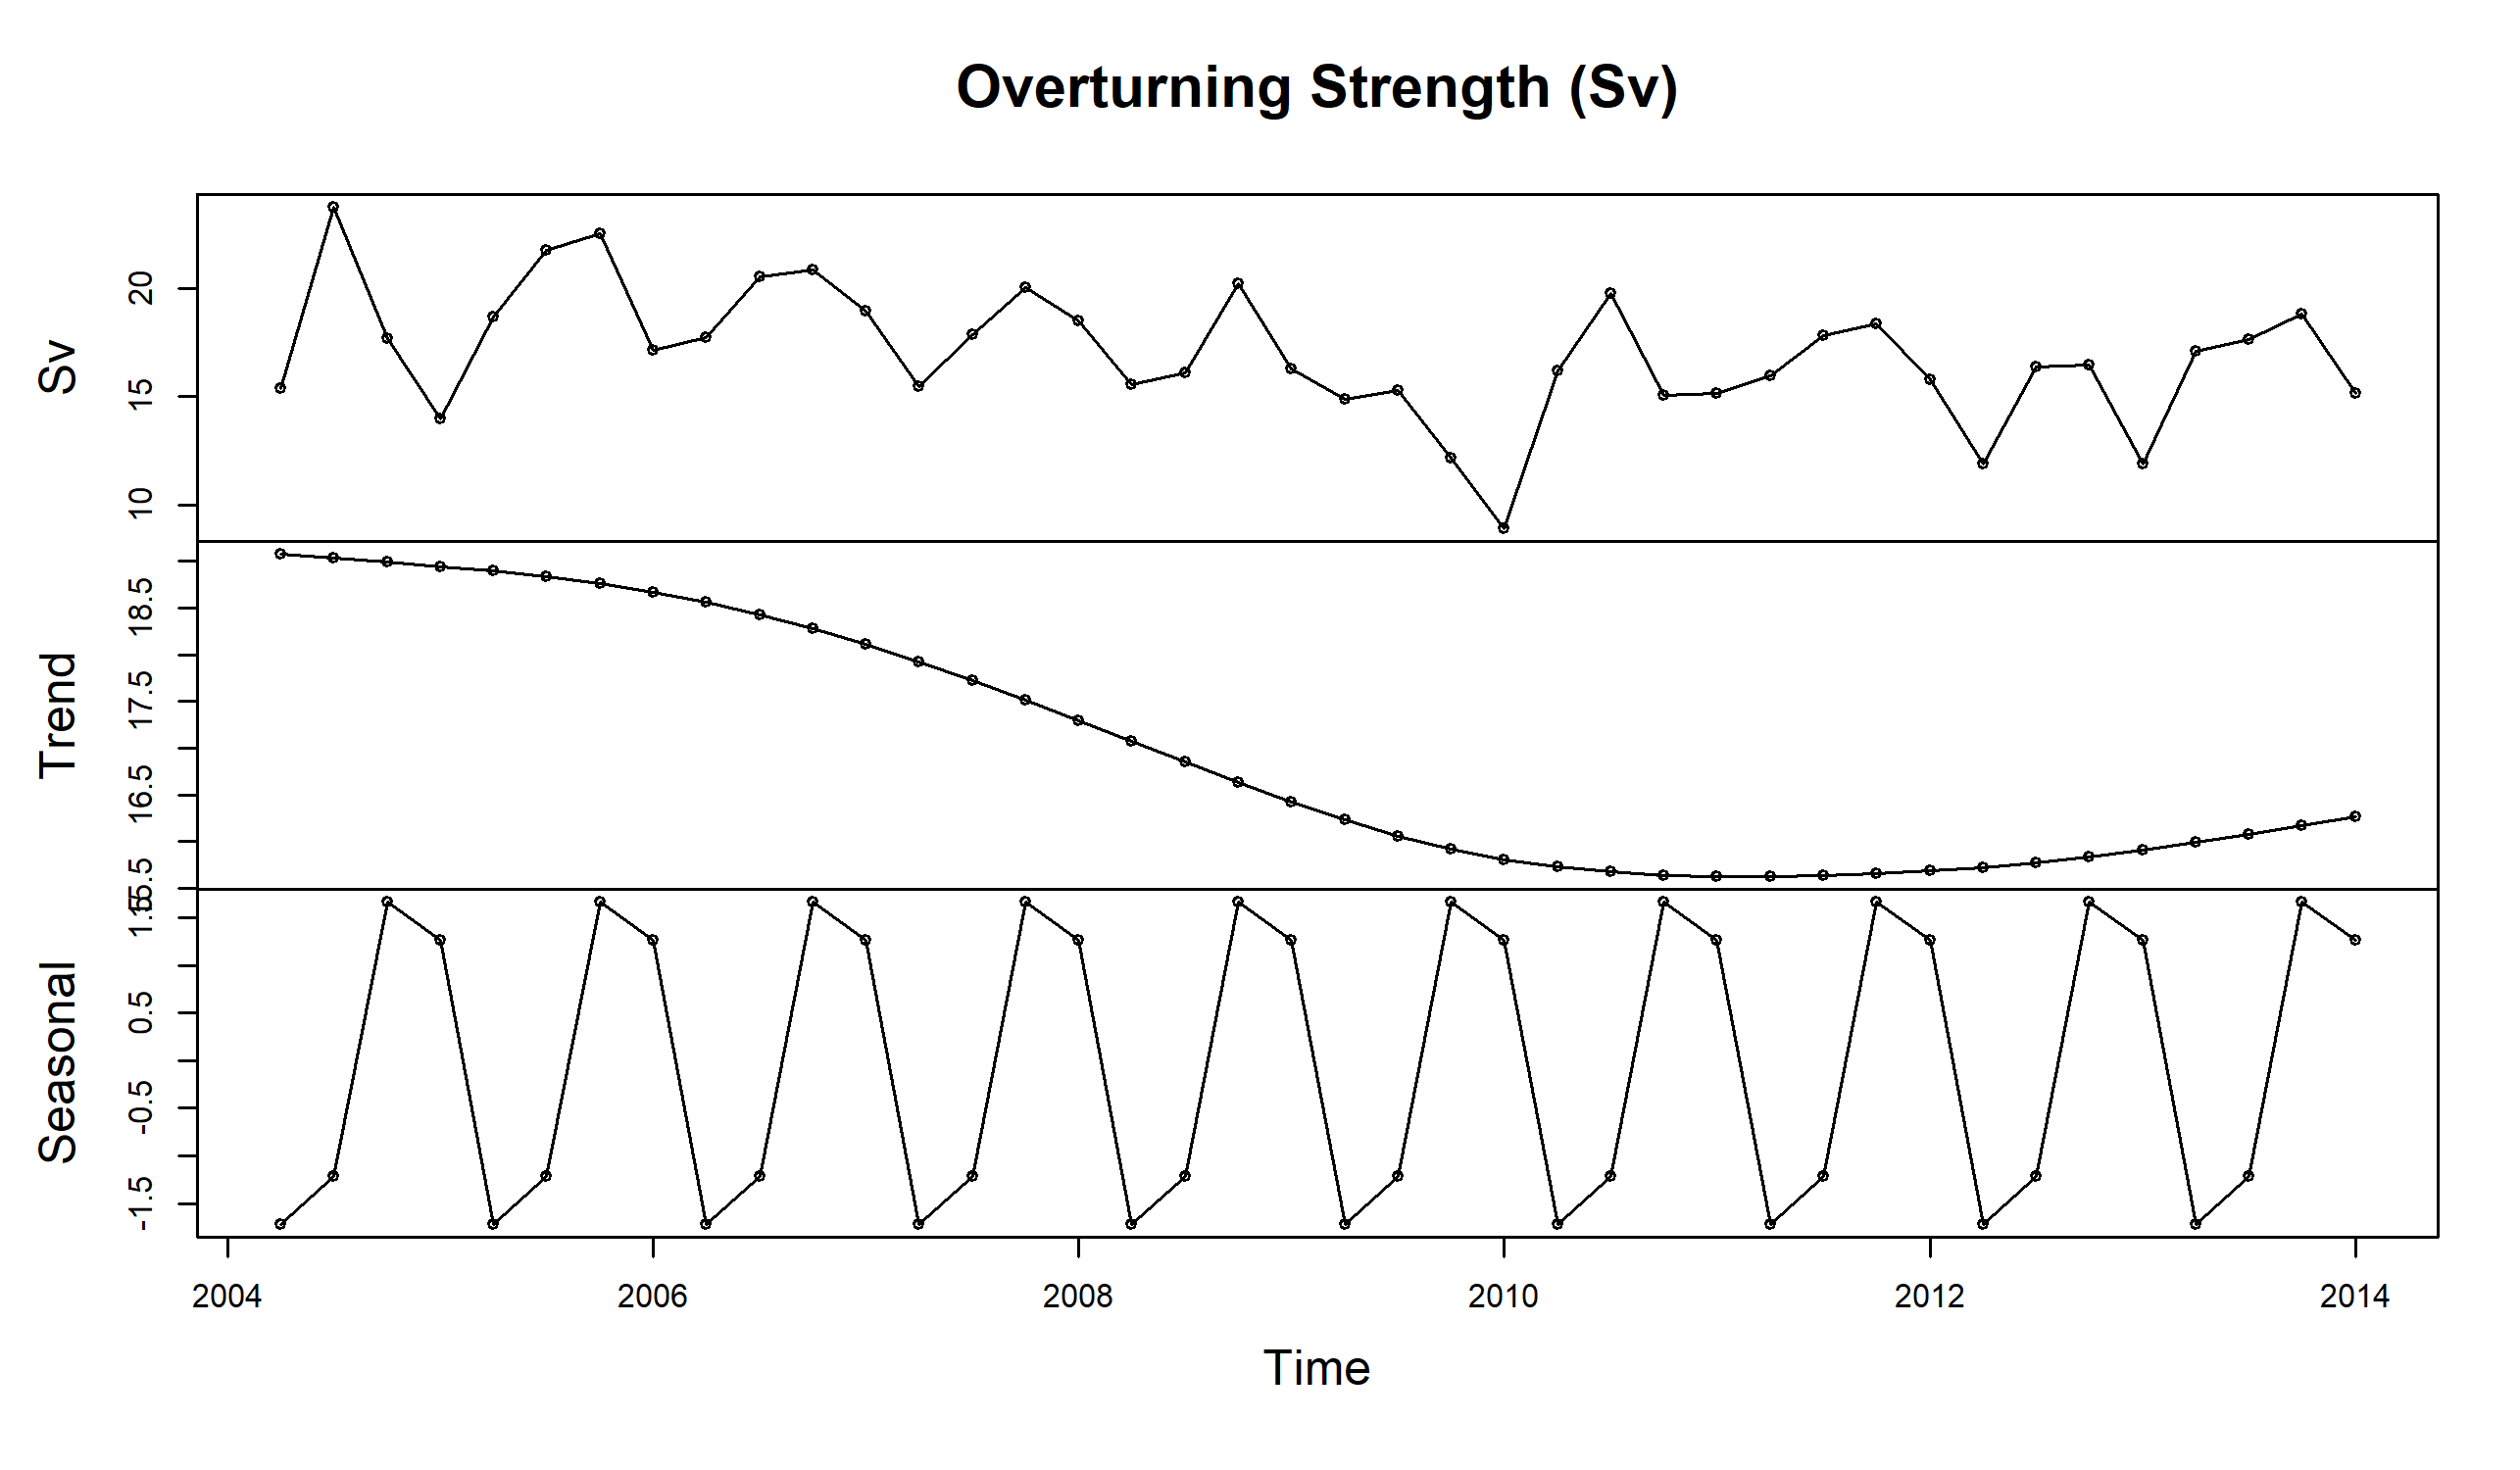
\includegraphics[width=0.60\textwidth]{Sections/DLM/Plots/trends.png}
    \caption{From top to bottom: The observed overturning strength, the estimated trend of our data from our model, the estimated seasonal component of data from our model.}
    \label{S3fig:trend}
\end{figure}

\begin{figure}[H]
    \centering
    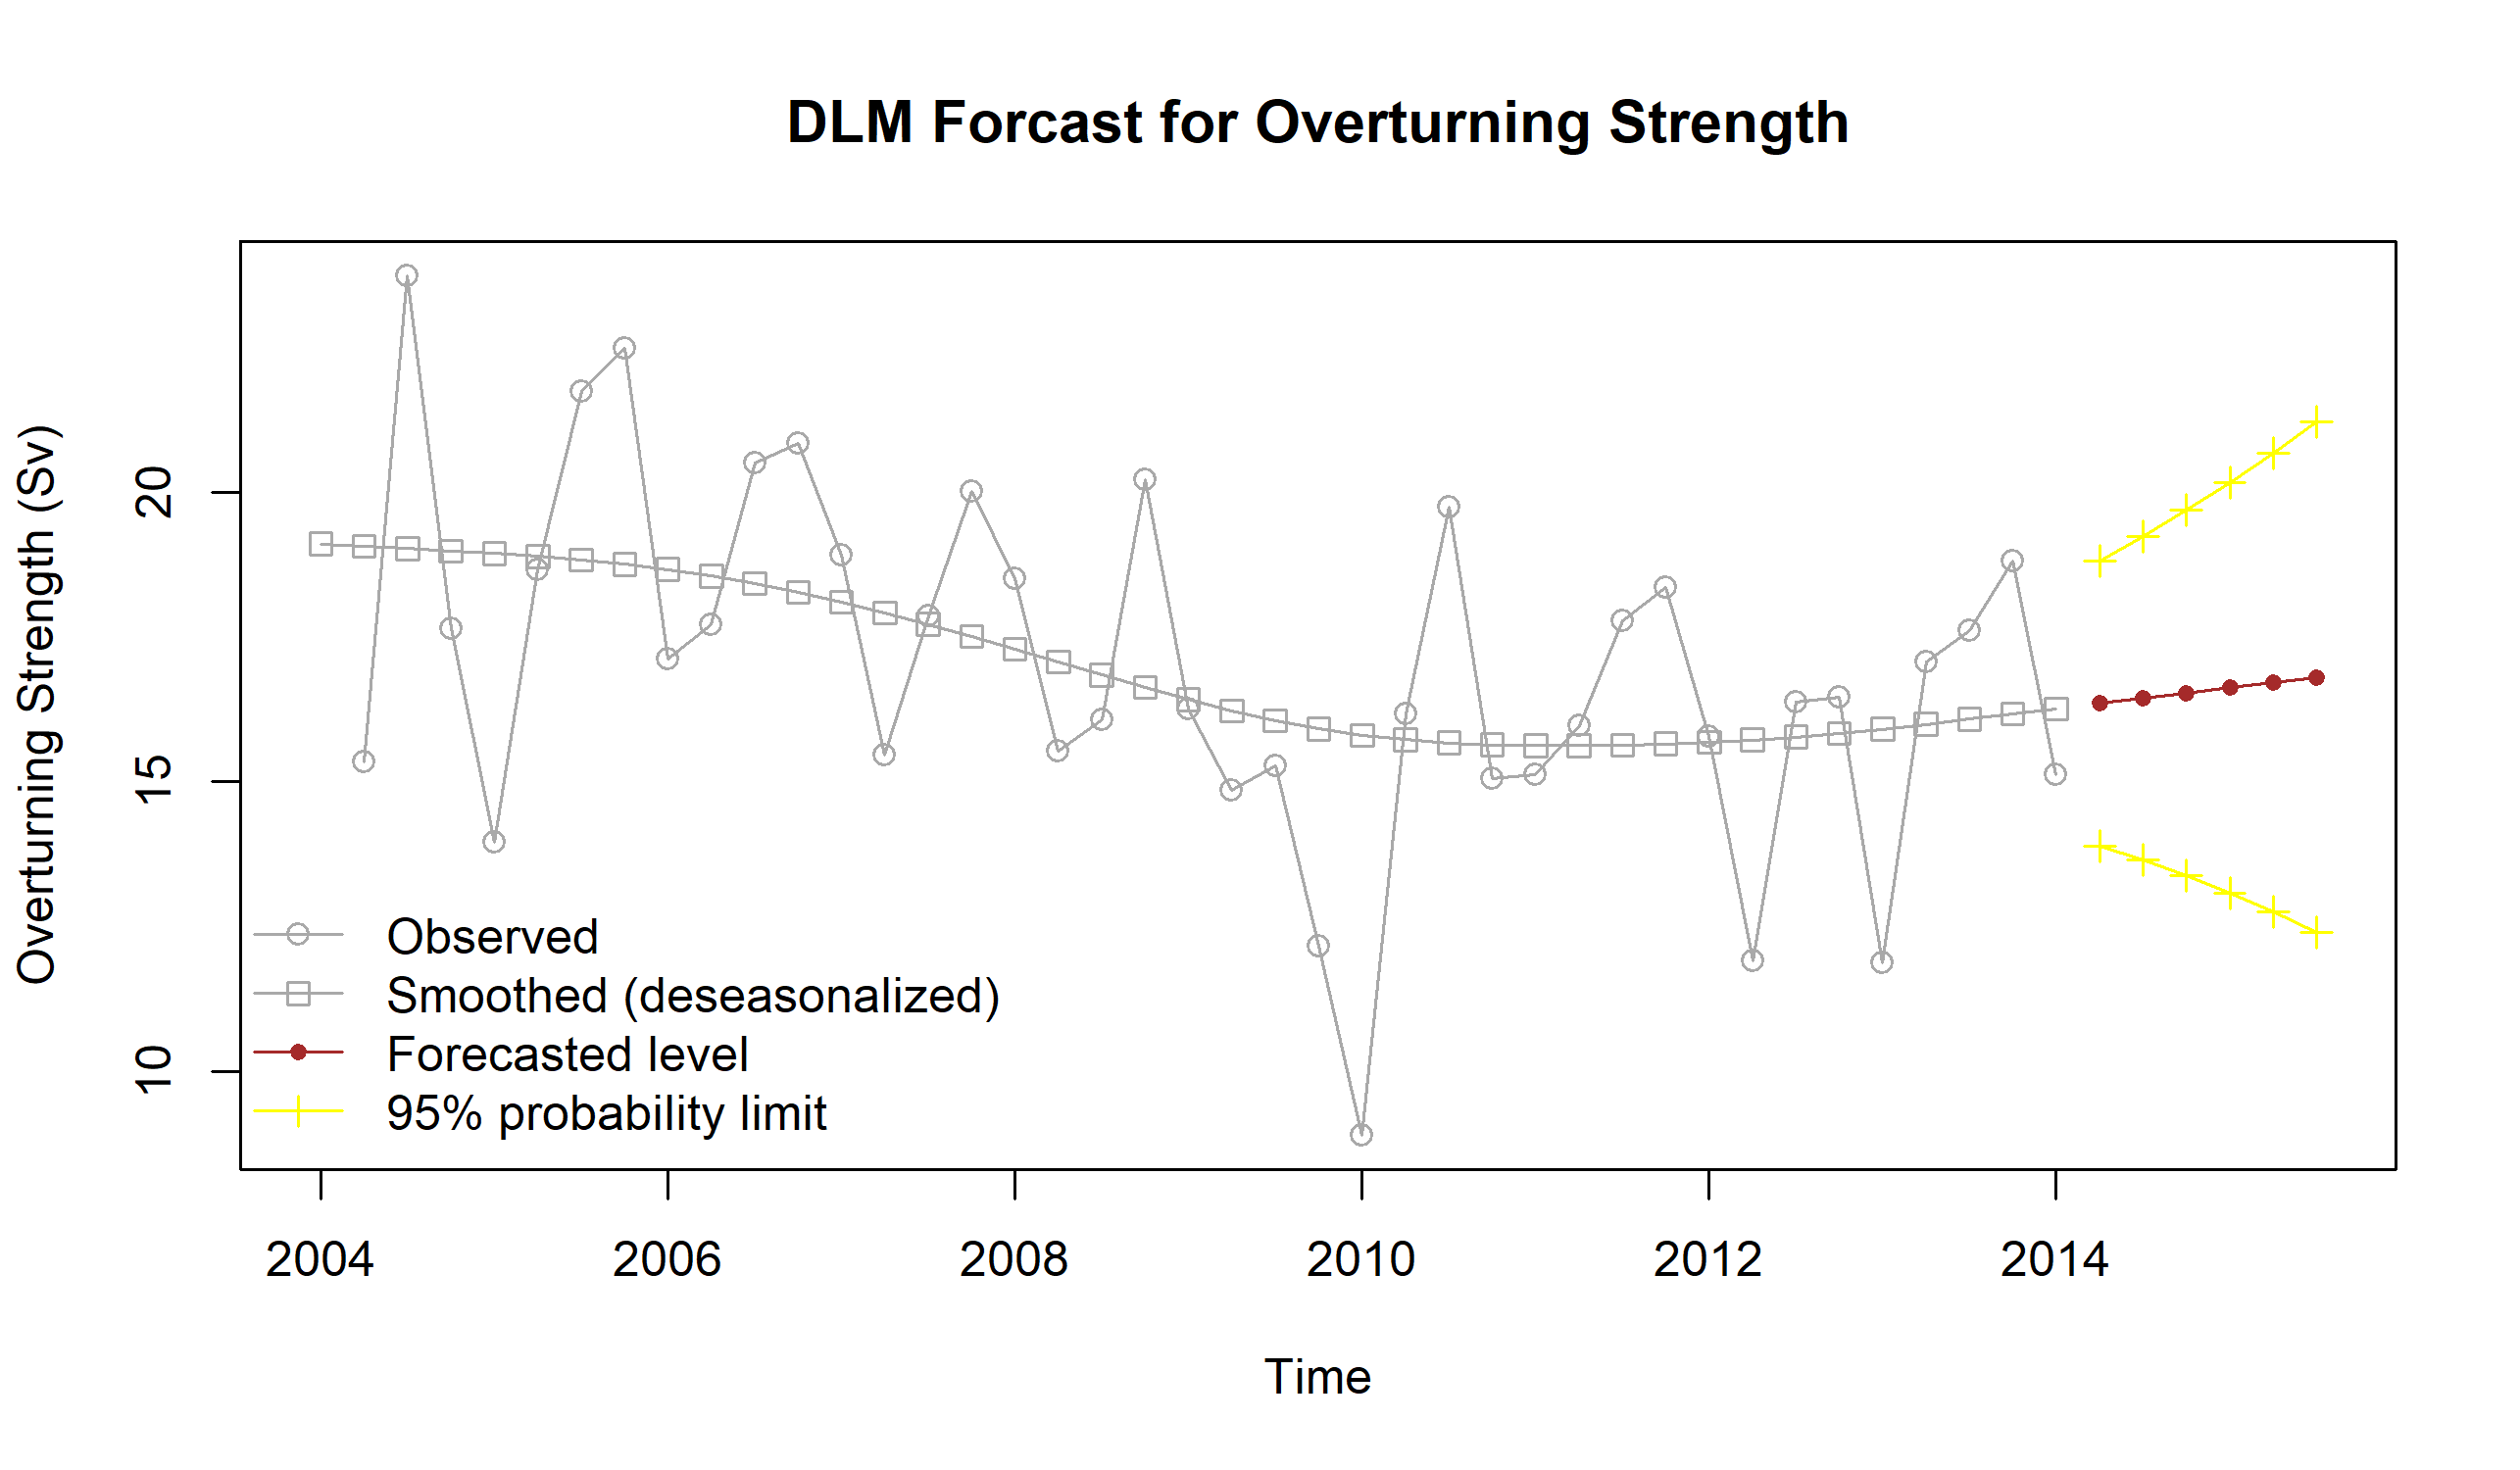
\includegraphics[width=0.60\textwidth]{Sections/DLM/Plots/forecast.png}
    \caption{Forecast of overturning strength (Sv) 6 quarters into the future with 95\% confidence intervals shown in yellow.}
    \label{S3fig:Forecast}
\end{figure}